\documentclass[aspectratio=43,17pt]{beamer} % or 14 or 17 or 20

\usepackage{tikz,pgf,lmodern,textpos,hyperref,graphicx,booktabs,appendixnumberbeamer,cleveref,fancybox,multicol}
\usepackage{pgfcalendar,svg,subfiles,chronosys,cancel,xcolor,color,nth,datenumber,xparse,fp,stackengine,makecell}
\usepackage{enumitem}
\usepackage{marvosym} % \MVRIGHTarrow
\usepackage{amsmath}
\usepackage{centernot}
\usetikzlibrary{positioning}
\usepackage[outline]{contour}
\usepackage[citestyle=authoryear-comp,backend=bibtex]{biblatex}
\usepackage[export]{adjustbox}
\usepackage[en-US]{datetime2}
\usepackage[normalem]{ulem}
\bibliography{references}
\usetheme[numbering=none]{metropolis}

\setlist[itemize]{label={--}}
% \setlist[itemize]{leftmargin=*}

% \bibliography{references}

%!TEX Root = ./presentation.tex

\definecolor{Blue}{HTML}{00548f}
\definecolor{Cardinal Red}{HTML}{8c1515}
\definecolor{White}{HTML}{ffffff}
\definecolor{Cool Grey}{HTML}{4d4f53}
\definecolor{Black}{HTML}{2e2d29}
\definecolor{Bright Red}{HTML}{B1040E}
\definecolor{Dark Red}{HTML}{820000}
\definecolor{Chocolate}{HTML}{2F2424}
\definecolor{Stone}{HTML}{544948}
\definecolor{Fog}{HTML}{F4F4F4}
\definecolor{Light Sandstone}{HTML}{F9F6EF}
\definecolor{Sandstone}{HTML}{d2c295}
\definecolor{Warm Grey}{HTML}{3f3c30}
\definecolor{Beige}{HTML}{9d9573}
\definecolor{Light Sage}{HTML}{c7d1c5}
\definecolor{Clay}{HTML}{5f574f}
\definecolor{Cloud}{HTML}{dad7cb}
\definecolor{Driftwood}{HTML}{b6b1a9}
\definecolor{Stone}{HTML}{928b81}
\definecolor{Sandhill}{HTML}{b3995d}
\definecolor{Palo Alto}{HTML}{175e54}
\definecolor{Teal}{HTML}{00505c}
\definecolor{Purple}{HTML}{53284f}
\definecolor{Redwood}{HTML}{8d3c1e}
\definecolor{Brown}{HTML}{5e3032}
\definecolor{Sky}{HTML}{0098db}
\definecolor{Lagunita}{HTML}{007c92}
\definecolor{Mint}{HTML}{009b76}
\definecolor{Gold}{HTML}{b26f16}
\definecolor{Sun}{HTML}{eaab00}
\definecolor{Poppy}{HTML}{e98300}

\definecolor{USF Green}{HTML}{00543C}
\definecolor{USF Gold}{HTML}{FDBB30}
\definecolor{USF Grey}{HTML}{919194}
% \definecolor{USF }{HTML}{e98300}


\setbeamercolor{normal text}{fg=Black,bg=White}
\hypersetup{colorlinks,linkcolor=USF Green,urlcolor=USF Green,citecolor=USF Green}
% \setbeamercolor{frametitle}{bg=Cardinal Red, fg=Blue}


\setbeamercolor{palette primary}{bg=Fog, fg=USF Green}
\setbeamercolor{palette secondary}{bg=USF Green, fg=Fog}
\setbeamercolor{frametitle}{bg=Fog,fg=USF Green}

% \setbeamercolor{section title}{fg=Dark Red, bg=Fog}
\setbeamercolor{alerted text}{fg=USF Green}

\newcommand{\soutthick}[1]{%
    \renewcommand{\ULthickness}{2.4pt}%
       \sout{#1}%
    \renewcommand{\ULthickness}{.4pt}% Resetting to ulem default
}


  \setbeamercolor{normal text}{%
    fg=Cool Grey,
    bg=White
  }

\setbeamercolor{palette primary}{fg=Fog, bg=Dark Red}
\setbeamercolor{palette secondary}{bg=Dark Red, bg=Fog}
\setbeamercovered{transparent}
% \setbeamercolor{background canvas}{bg=Fog}
\setbeamercolor{frametitle}{bg=Dark Red,fg=Fog}
\hypersetup{colorlinks,linkcolor=Blue,urlcolor=Blue,citecolor=Blue}
\setbeamercolor{alerted text}{fg=Bright Red}
\setbeamertemplate{caption}{\insertcaption}


\setsansfont[BoldFont={Source Sans Pro Bold},
              Numbers={OldStyle}]{Source Sans Pro}
\setmainfont[BoldFont={Source Serif Pro Semibold},
              Numbers={OldStyle}]{Source Serif Pro}
\setmonofont{Source Code Pro}


\metroset{titleformat=smallcaps,numbering=none}


\newenvironment{mystepwiseitemize}{\begin{itemize}[<+-| alert@+>]}{\end{itemize}}




\title{Data Ethics Lecture 5}
\subtitle{Philosophical foundations}
\author[Ali Alkhatib]{{Ali Alkhatib}\\
\href{http://twitter.com/_alialkhatib}{@\_alialkhatib} || \href{mailto:hi@al2.in}{hi@al2.in}}
\date{March April 7, 2022}

% \date{\today}


\newcommand{\onlyinsubfile}[1]{#1}
\newcommand{\notinsubfile}[1]{}

\begin{document}
\renewcommand{\onlyinsubfile}[1]{}
\renewcommand{\notinsubfile}[1]{#1}


\begin{frame}
\titlepage
\end{frame}

\begin{frame}\frametitle{Roadmap for today}


\visible<+->{\begin{columns}
\begin{column}{0.5\textwidth}
This week \hfill \MVRightarrow{}
\end{column}
\begin{column}{0.4\textwidth}
\strong{Philosophical foundations}
\end{column}
\end{columns}}

\vspace{2em}

\visible<+->{\begin{columns}
\begin{column}{0.5\textwidth}
Next week \hfill \MVRightarrow{}
\end{column}
\begin{column}{0.4\textwidth}
\strong{Organizing and Activism}
\end{column}
\end{columns}}



\end{frame}

\section{Philosophical foundations}

\begin{frame}[t]{foundations}
    We've talked about a few philosophical approaches before\only<+>{:}
    
    \only<.>{\begin{itemize}
            \item consequentialism
            \item deontology
            \item virtue ethics
        \end{itemize}}

\only<+->{we're going to add a few other frameworks

\begin{itemize}
    \item colonialism
    \item restorative justice
    \item harm reduction
\end{itemize}
}

\end{frame}

\begin{frame}{philosophy}


\begin{columns}
\begin{column}{0.5\textwidth}

\visible<+->{\small\begin{itemize}[itemsep=0em]
    
    \item<alert@+> consequentialism
    
    \item<alert@+> deontology
    
    \item<alert@+> virtue ethics
    
    \item<alert@+> colonialism
    
    \item<alert@+> restorative justice
    
    \item<alert@+> harm reduction

\end{itemize}}

\end{column}

\begin{column}{0.5\textwidth}

\only<5>{\includegraphics[width=\textwidth]{figures/papers/algo_colonization_africa2.png}}

\only<6>{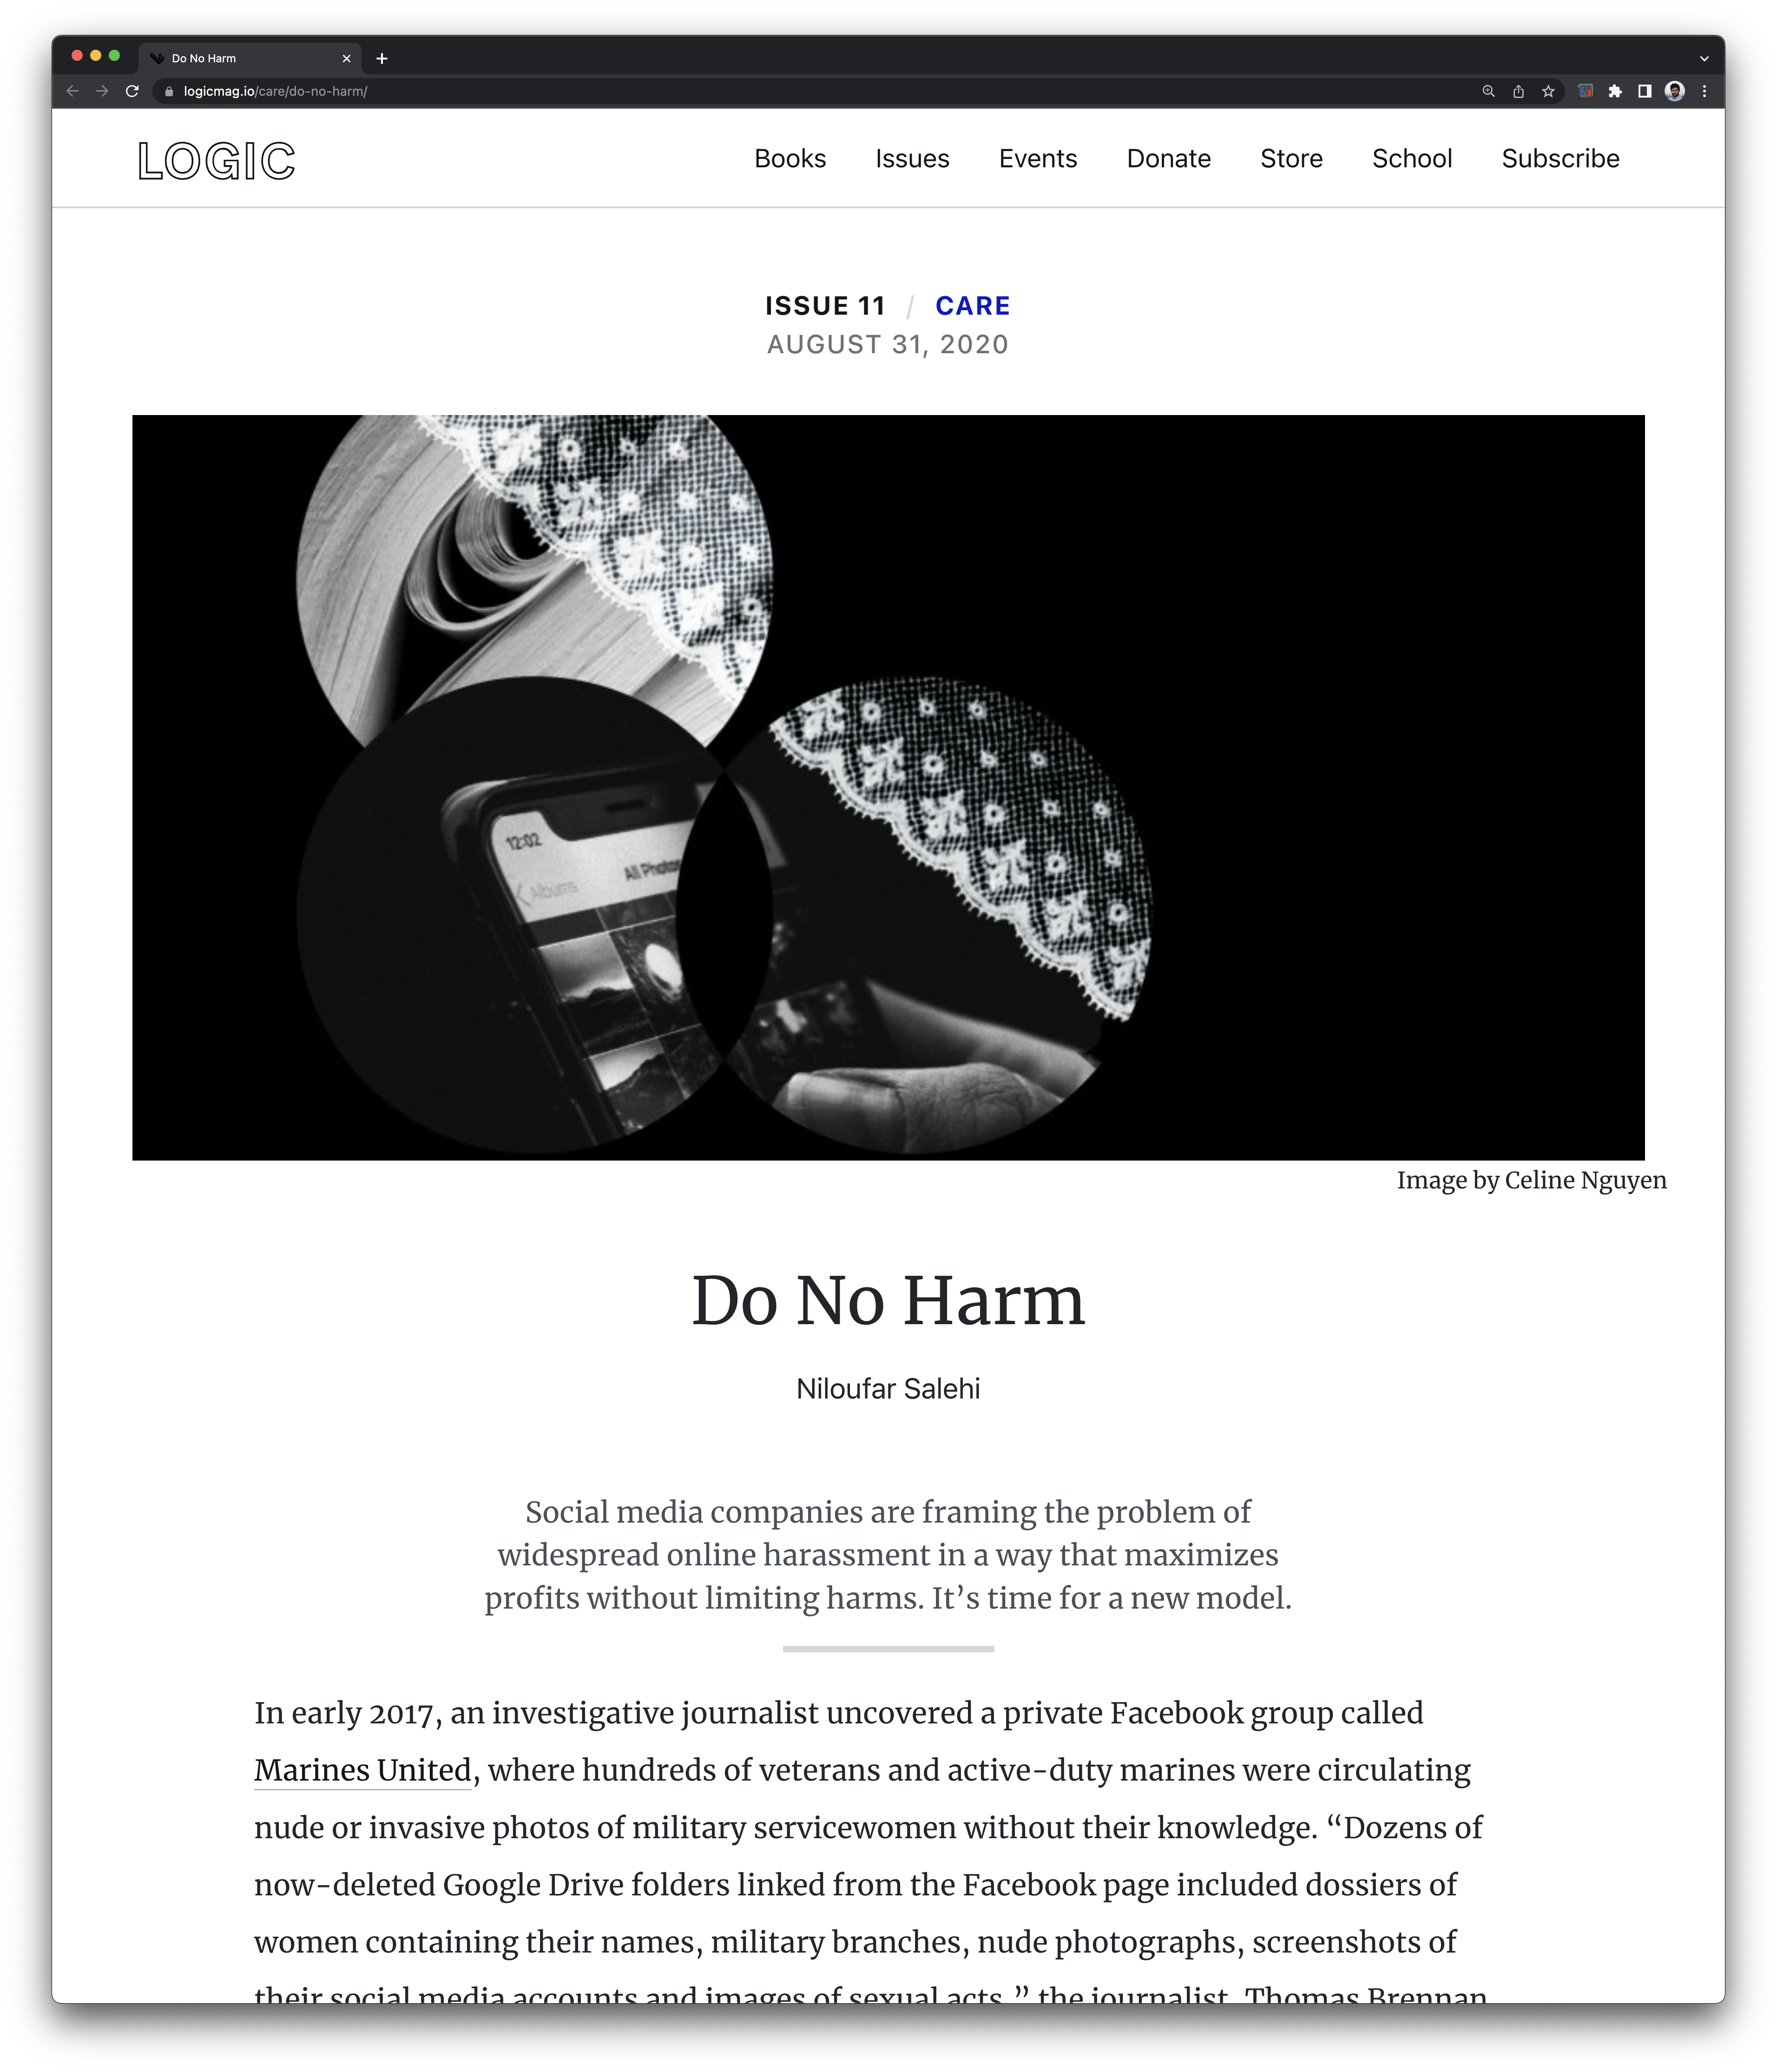
\includegraphics[width=\textwidth]{figures/papers/restorative_justice_salehi.png}}


\end{column}
\end{columns}

\end{frame}

\end{document}
